\documentclass{article}

\usepackage[utf8]{inputenc}
\usepackage[ngerman]{babel}
\usepackage[T1]{fontenc}

\usepackage{amsmath}
\usepackage{amssymb}
\usepackage{amsthm}
\usepackage{bbm}

\usepackage{geometry}
\geometry{a4paper,left=3cm,right=3cm,top=2.5cm,bottom=2.5cm}

\renewcommand{\baselinestretch}{1.45} 
\usepackage{setspace}

\usepackage{multicol}

\usepackage{graphicx} %use graph format
\usepackage{epstopdf}


\title{Non-Paramatric Statistics Exercise 4}
\author{Osman Ceylan, Jiahui Wang, Zhuoyao Zeng}
\date{\today}

\begin{document}
\maketitle

\section*{Exercise 2.3} \vspace*{-1em}
Implement the histogram rule $h_{D,s}$ in an algorithm that only uses $O(n)$ spaces, where $n$ is the number of samples. Visualize the effect of different widths on the data sets of Exercise 2.2.\\
\textit{Solution: }\\
\textbf{Here we describe our implementation:}\\
Input is the data set $D$ of $n$ samples, a given point as origin for cell generation $(x_0,y_0)$ and the width of cells $s$.\\
Our algorithm identifies each cubic cell $A$ with its center $c_A$ and uses a dictionary to store $c_A$ as keys and the respective histogram values of each cell (as values of the dictionary). This data structure enables storage complexity to stay within $O(n)$.\\
\underline{Step 1}: For each cell $A$, the algorithm calculates $|\{ i\in \mathbb{N} : x_i\in A\}|$. \\
It means, that for each point $d \in D$ our algorithm determines $A(x)$ by a simple calculation and sees whether $c_{A(x)}$ is already a key in the dictionary. If $c_{A(x)}$ already exists in the dictionary, the value of $c_{A(x)}$ will increase 1; else the key $c_{A(x)}$ will be created and receives the value 1.\\
\underline{Step 2}: For each key $c_{A(x)}$ from the dictionary, the algorithm devides its value $|\{ i\in \mathbb{N} : x_i\in A\}|$ by $n * s^2$, so that the histogram values $h_{D,s}$ are generated. \\
\underline{Step 3}: The algorithm plots $c_{A(x)}$ as scatters and uses colours to represent different histogram values. The module $matplotlib.cm$ is deployed for the colour scheme. \\
\textbf{Now we present our graphical results for Exercise 2.2 $i)$:} \\
We draw 30,000 samples from the distribution $\mathbf{P}$ with \\
\begin{center} \vspace*{-0.8cm}
$\mathbf{P} \sim \frac{1}{3} N ( \bigl(\begin{smallmatrix} 0 \\ 3e \end{smallmatrix}\bigr), \bigl(\begin{smallmatrix} 5 & 0.5\\ 0.5 & 2 \end{smallmatrix}\bigr) ) + \frac{1}{3} N ( \bigl(\begin{smallmatrix} \pi \\ 1 \end{smallmatrix}\bigr), \bigl(\begin{smallmatrix} ln3 & 1.8\\ 1.8 & 5 \end{smallmatrix}\bigr) ) + \frac{1}{3} N ( \bigl(\begin{smallmatrix} -8 \\ -4 \end{smallmatrix}\bigr), \bigl(\begin{smallmatrix} ln3+5ln10 & 2\\ 2 & 6.6666 \end{smallmatrix}\bigr) )$.
\end{center} \ \vspace*{-0.7cm}\\
On the next page, we will finally show our results for Exercise 2.2 i). 
\newpage
For different choice of $s$, we obtained following different histograms: \\
\hspace*{-1.5cm}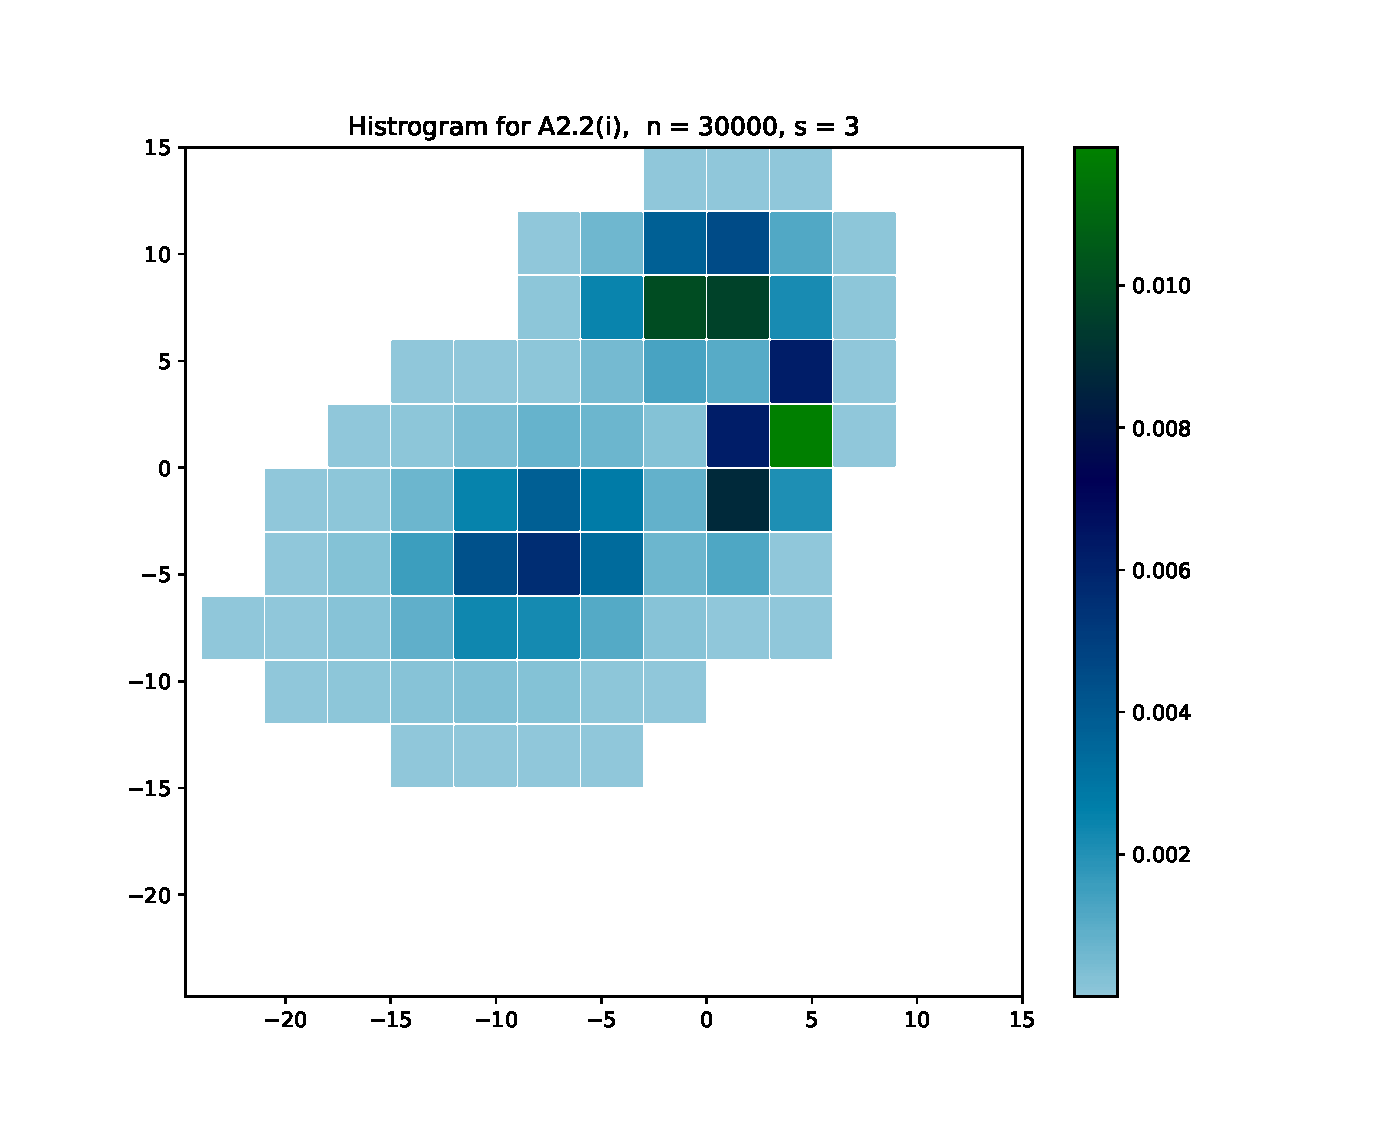
\includegraphics[height=8cm]{Figures_for_A2.2_i//1.eps} \hspace*{-1.5cm}
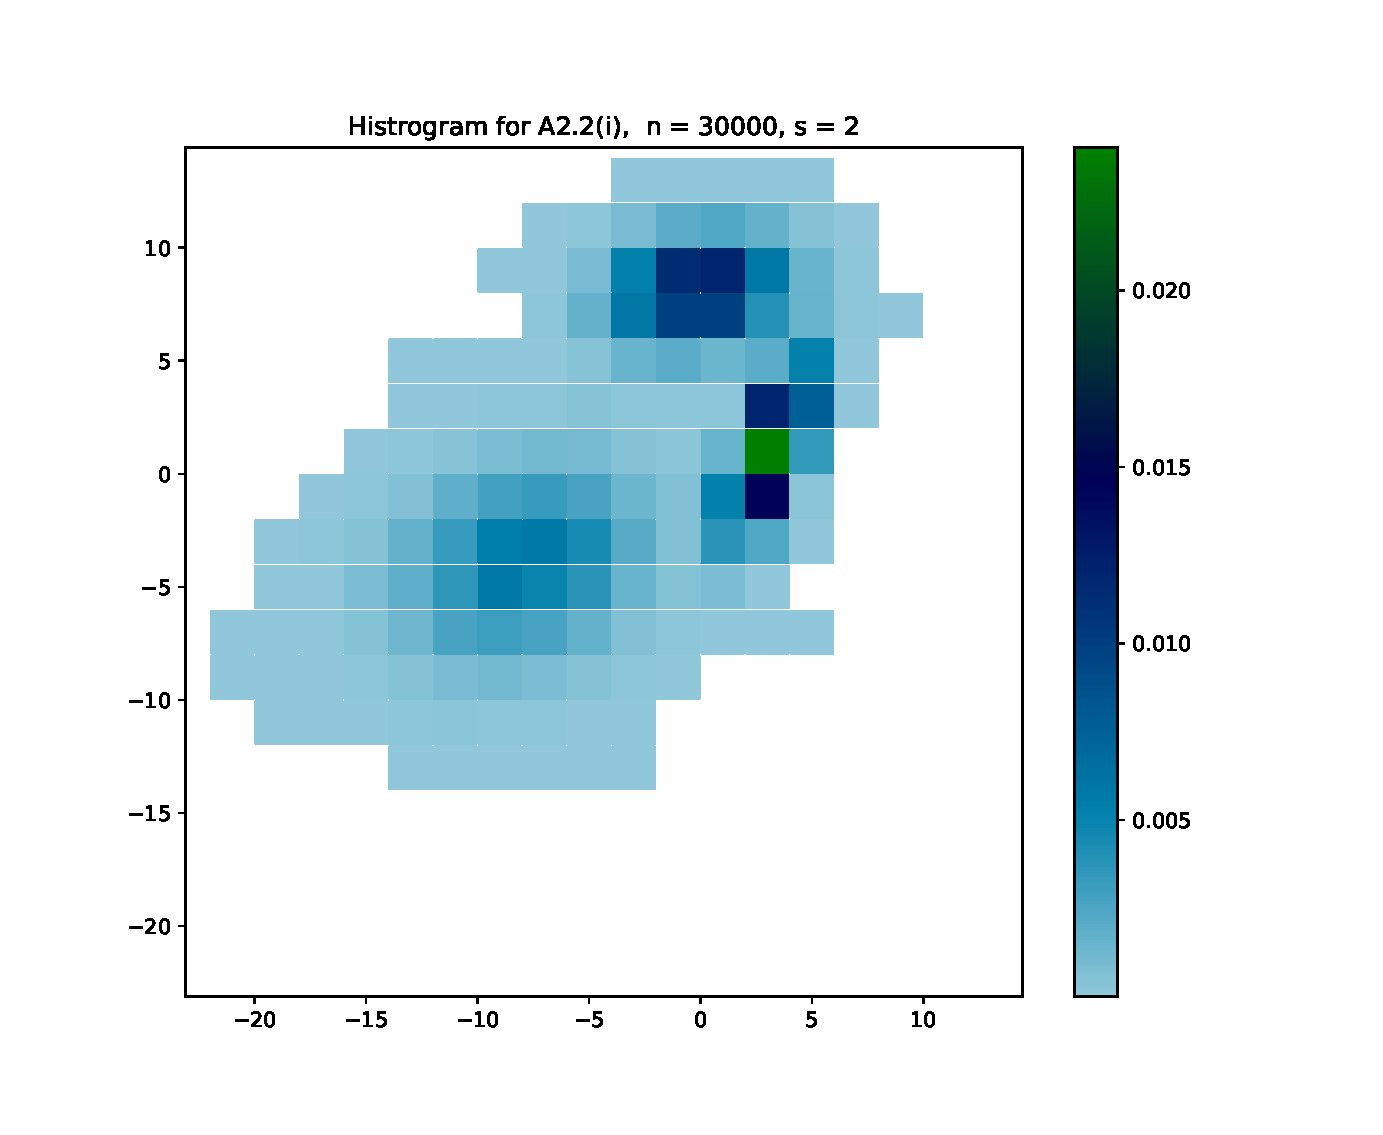
\includegraphics[height=8cm]{Figures_for_A2.2_i//2.eps}\\
\hspace*{-1.5cm}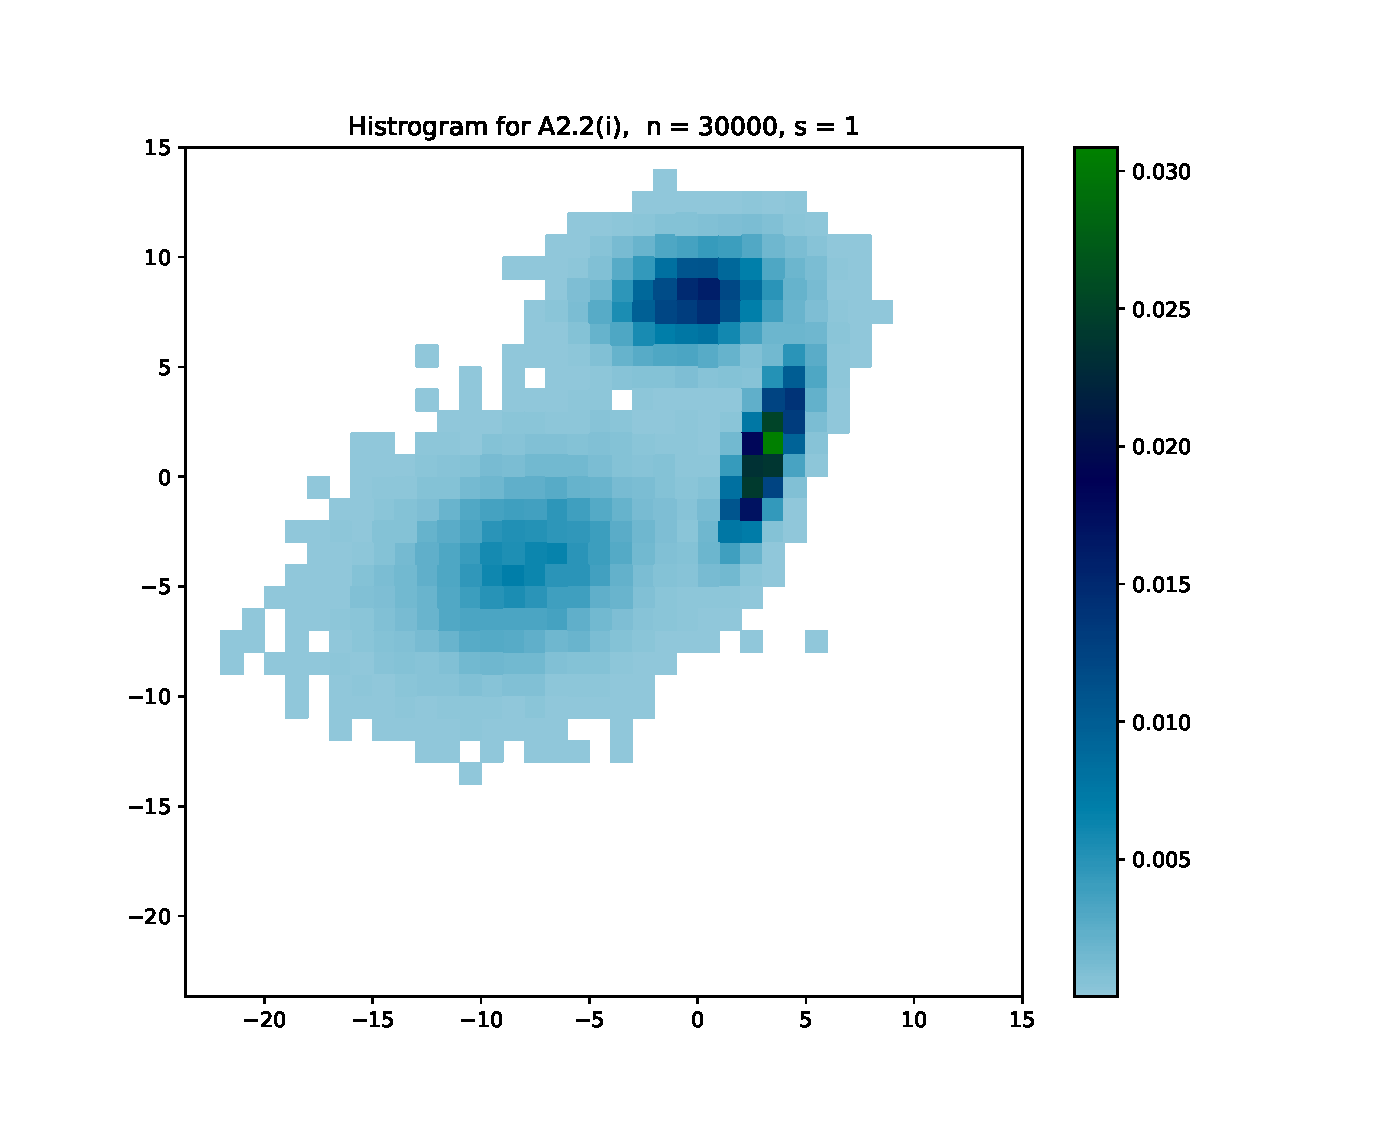
\includegraphics[height=8cm]{Figures_for_A2.2_i//3.eps} \hspace*{-1.5cm}
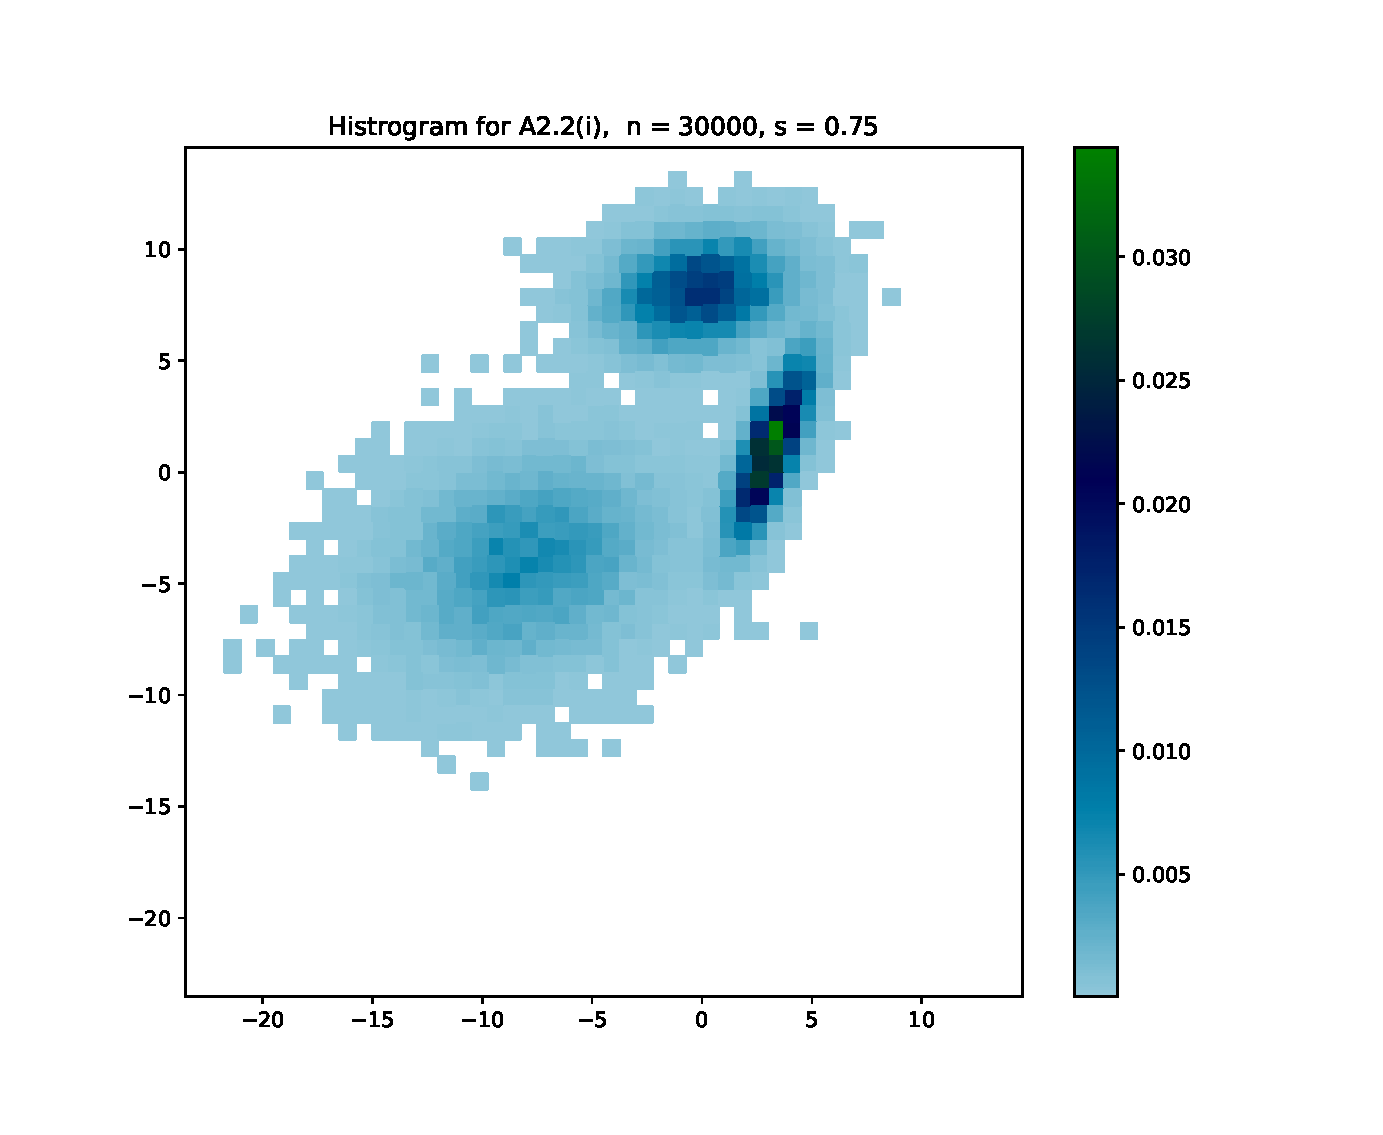
\includegraphics[height=8cm]{Figures_for_A2.2_i//4.eps}\\
\hspace*{-1.5cm}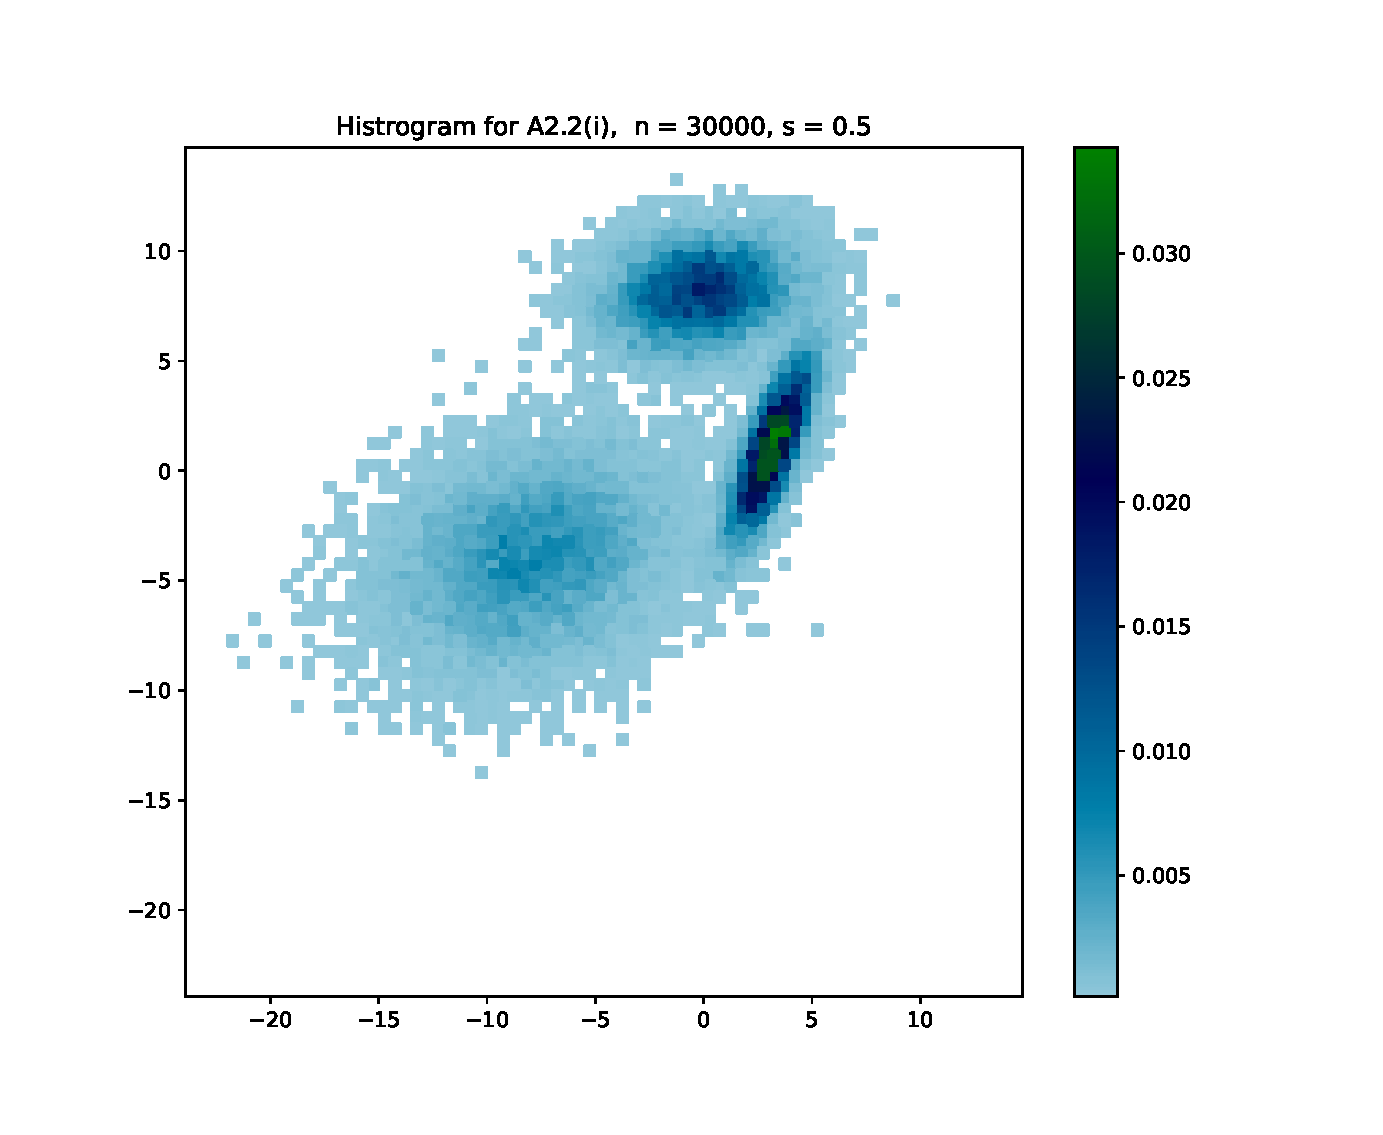
\includegraphics[height=8cm]{Figures_for_A2.2_i//5.eps} \hspace*{-1.5cm}
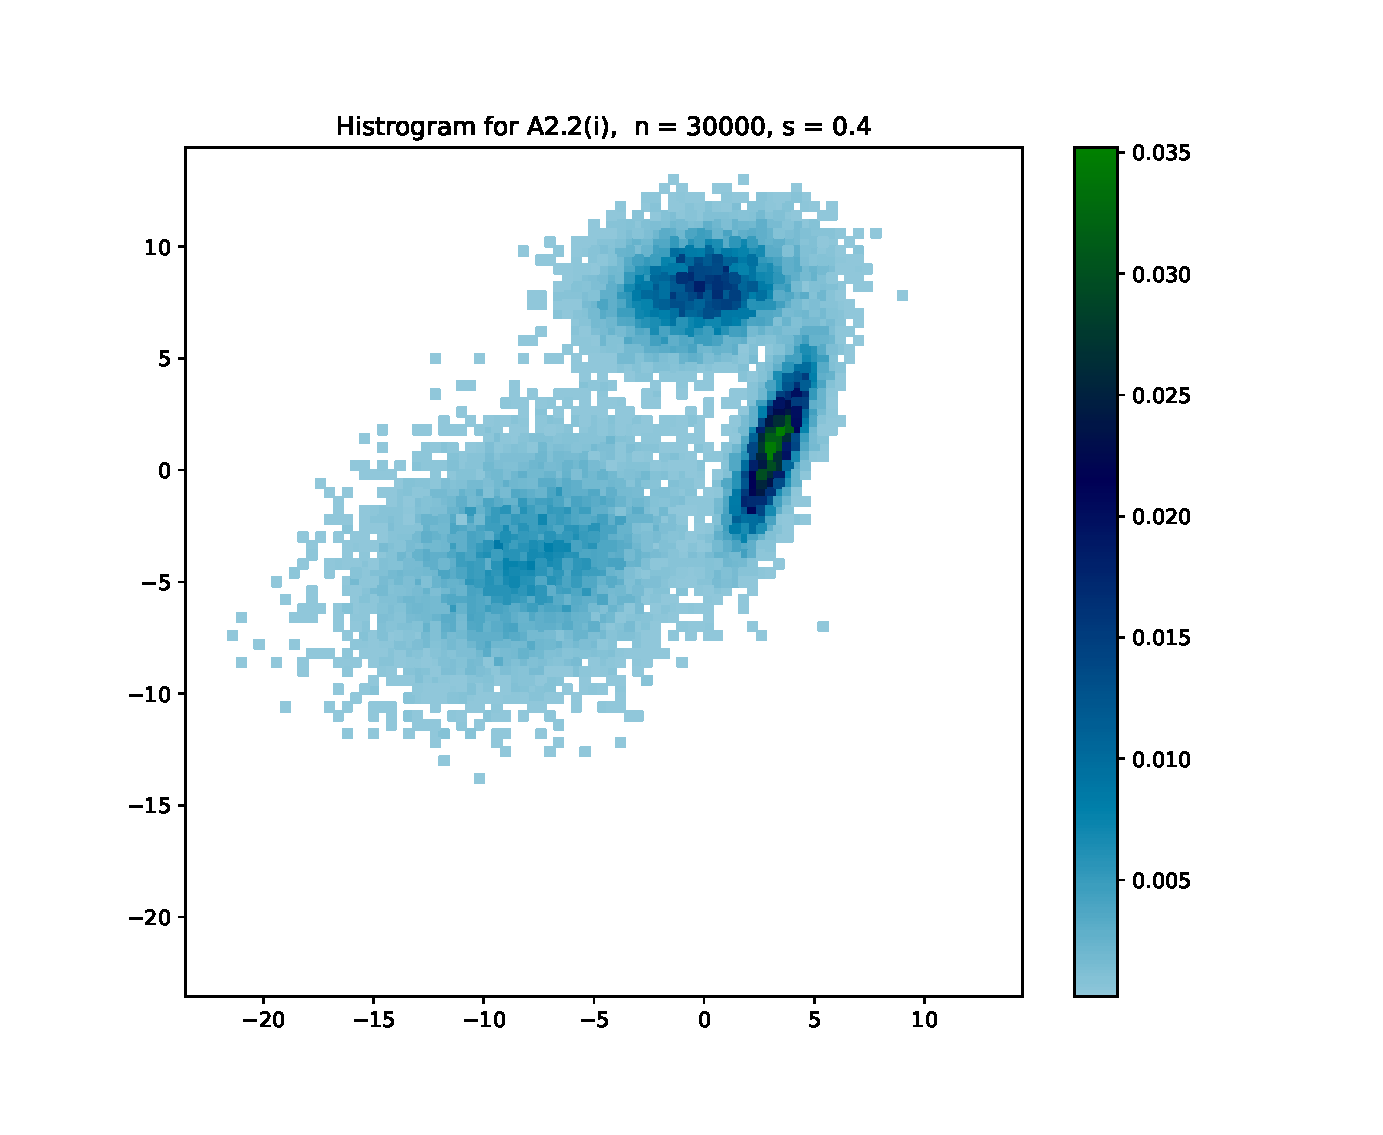
\includegraphics[height=8cm]{Figures_for_A2.2_i//6.eps}\\
\hspace*{-1.5cm}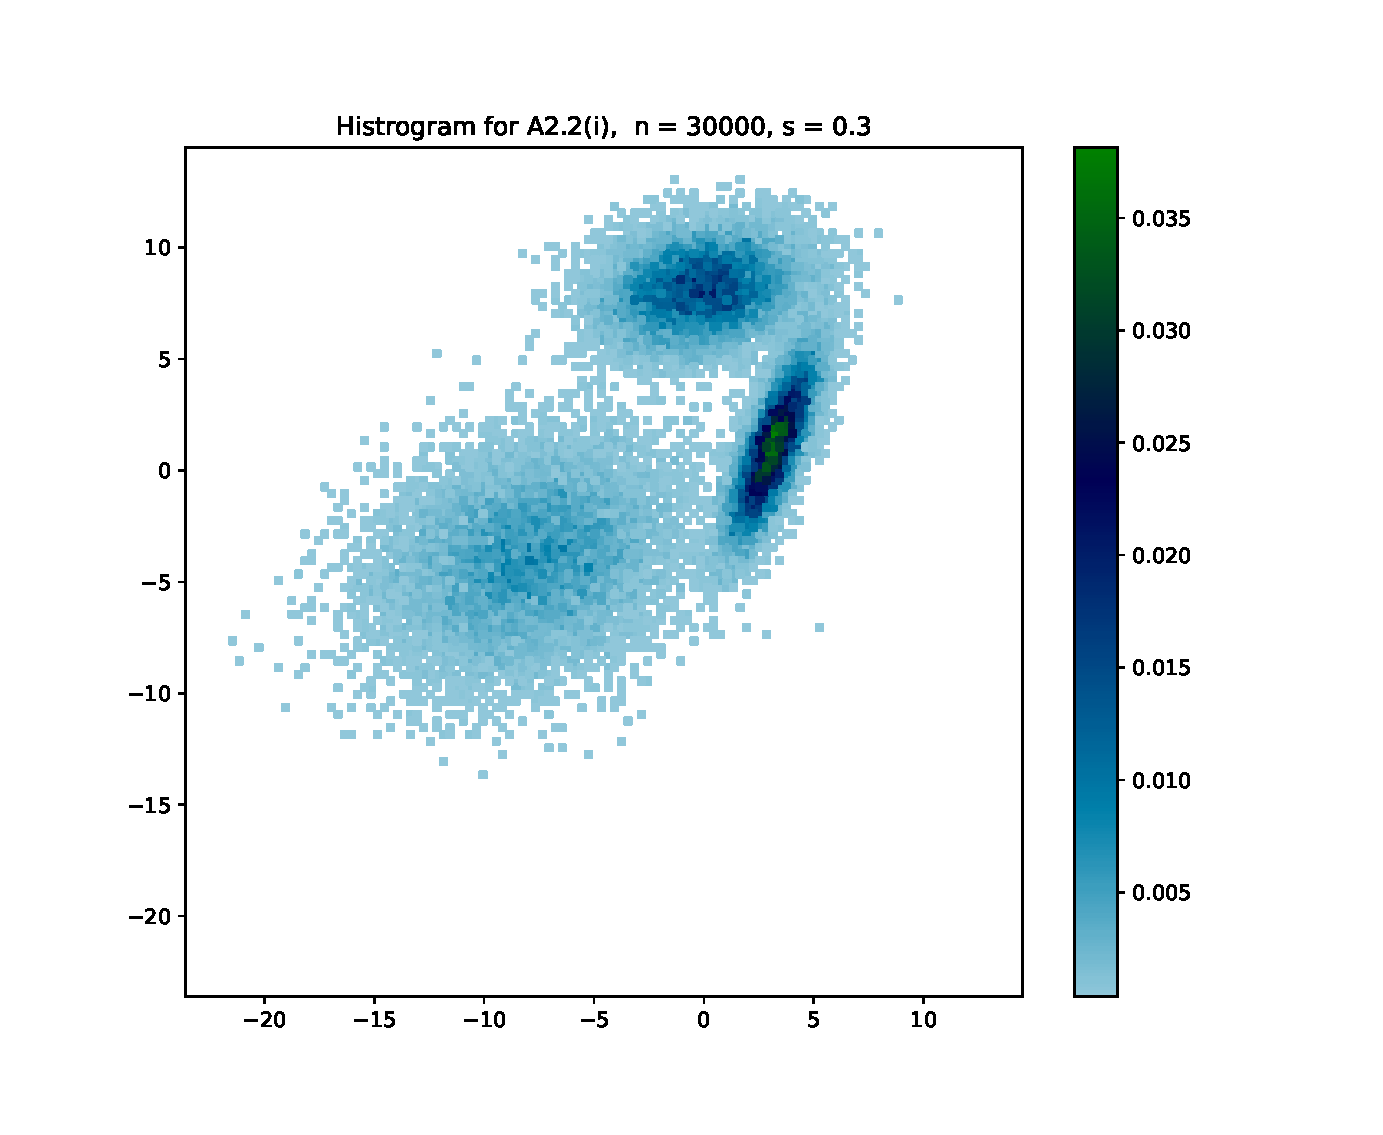
\includegraphics[height=8cm]{Figures_for_A2.2_i//7.eps} \hspace*{-1.5cm}
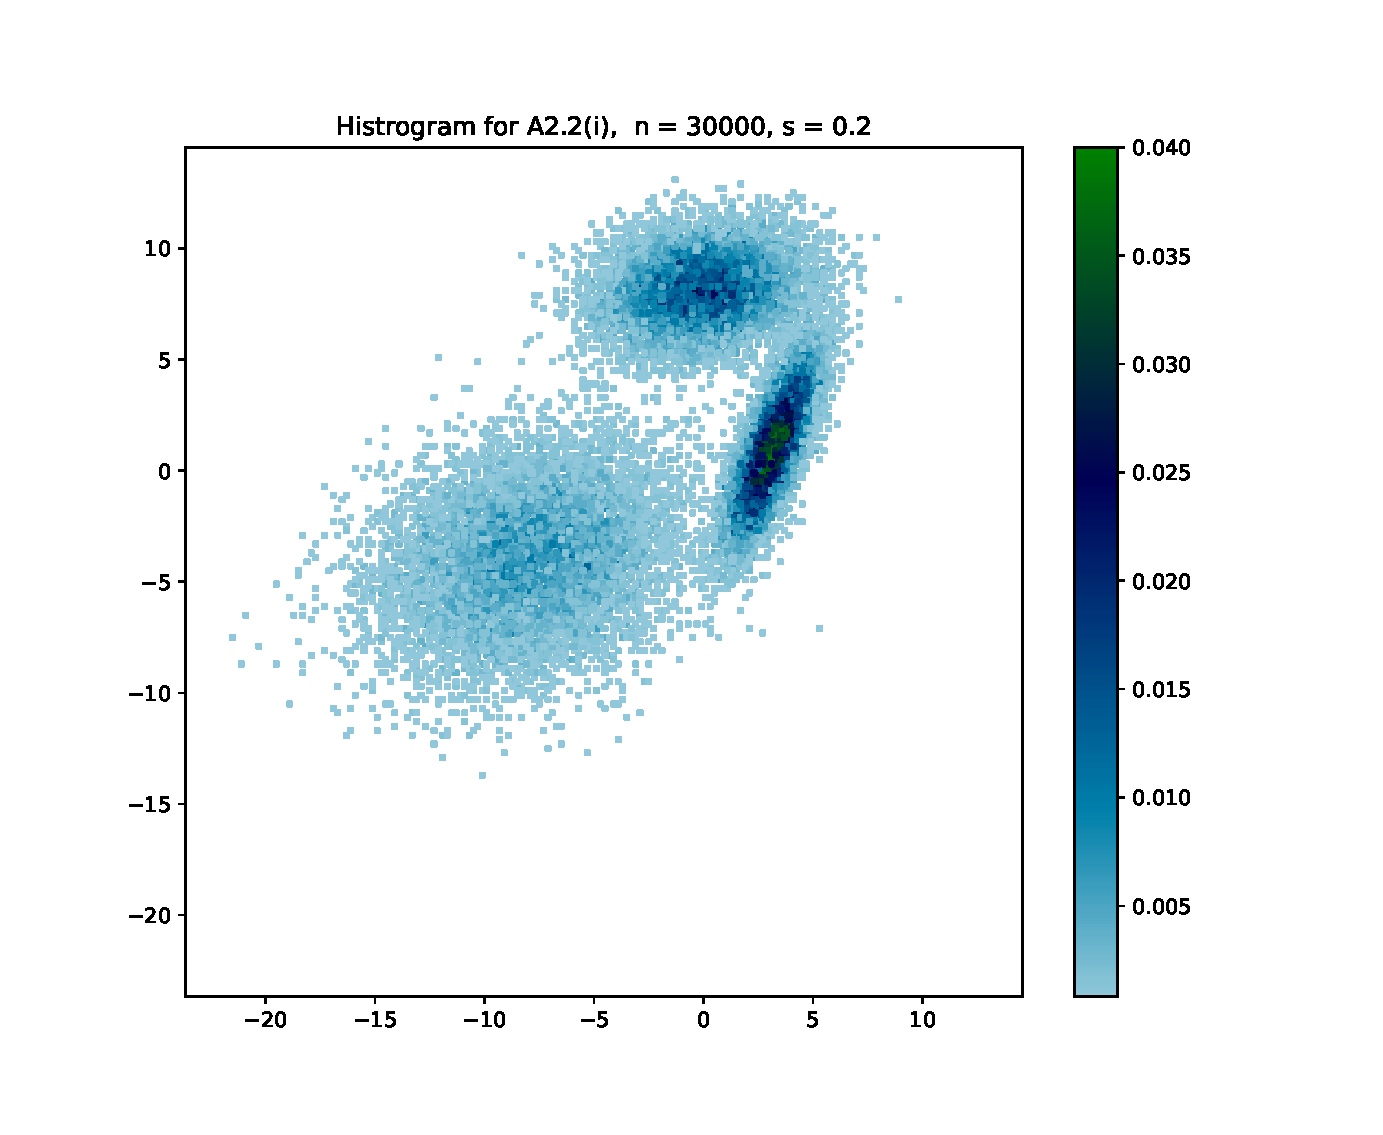
\includegraphics[height=8cm]{Figures_for_A2.2_i//8.eps}\\
\hspace*{-1.5cm}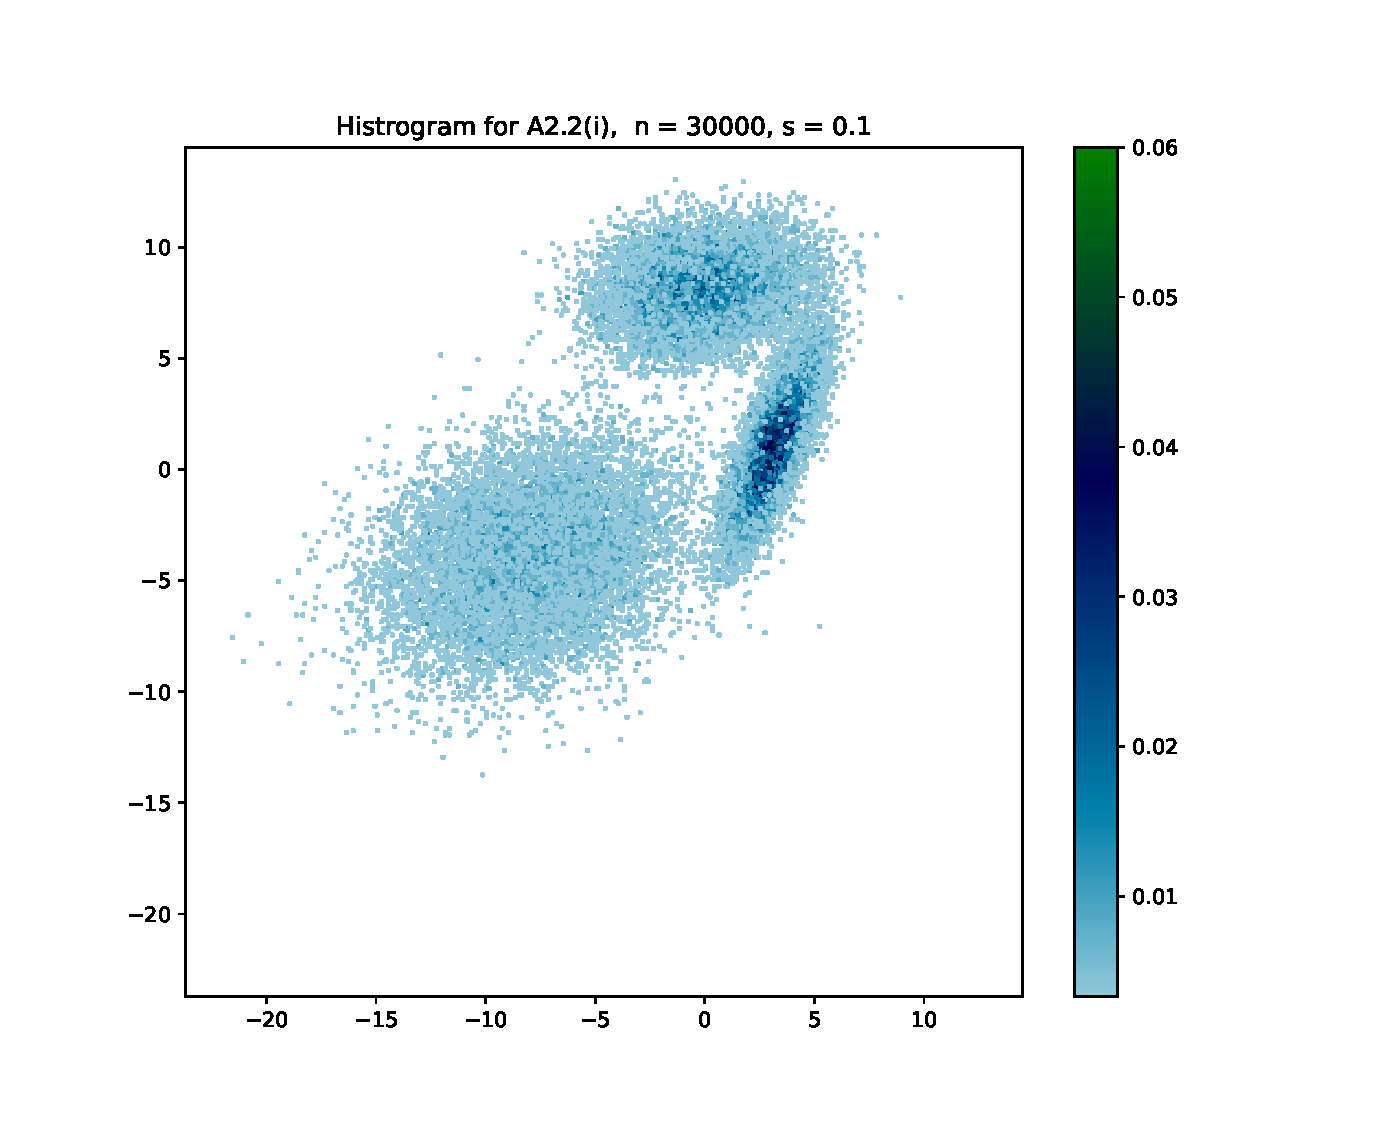
\includegraphics[height=8cm]{Figures_for_A2.2_i//9.eps} \hspace*{-1.5cm}
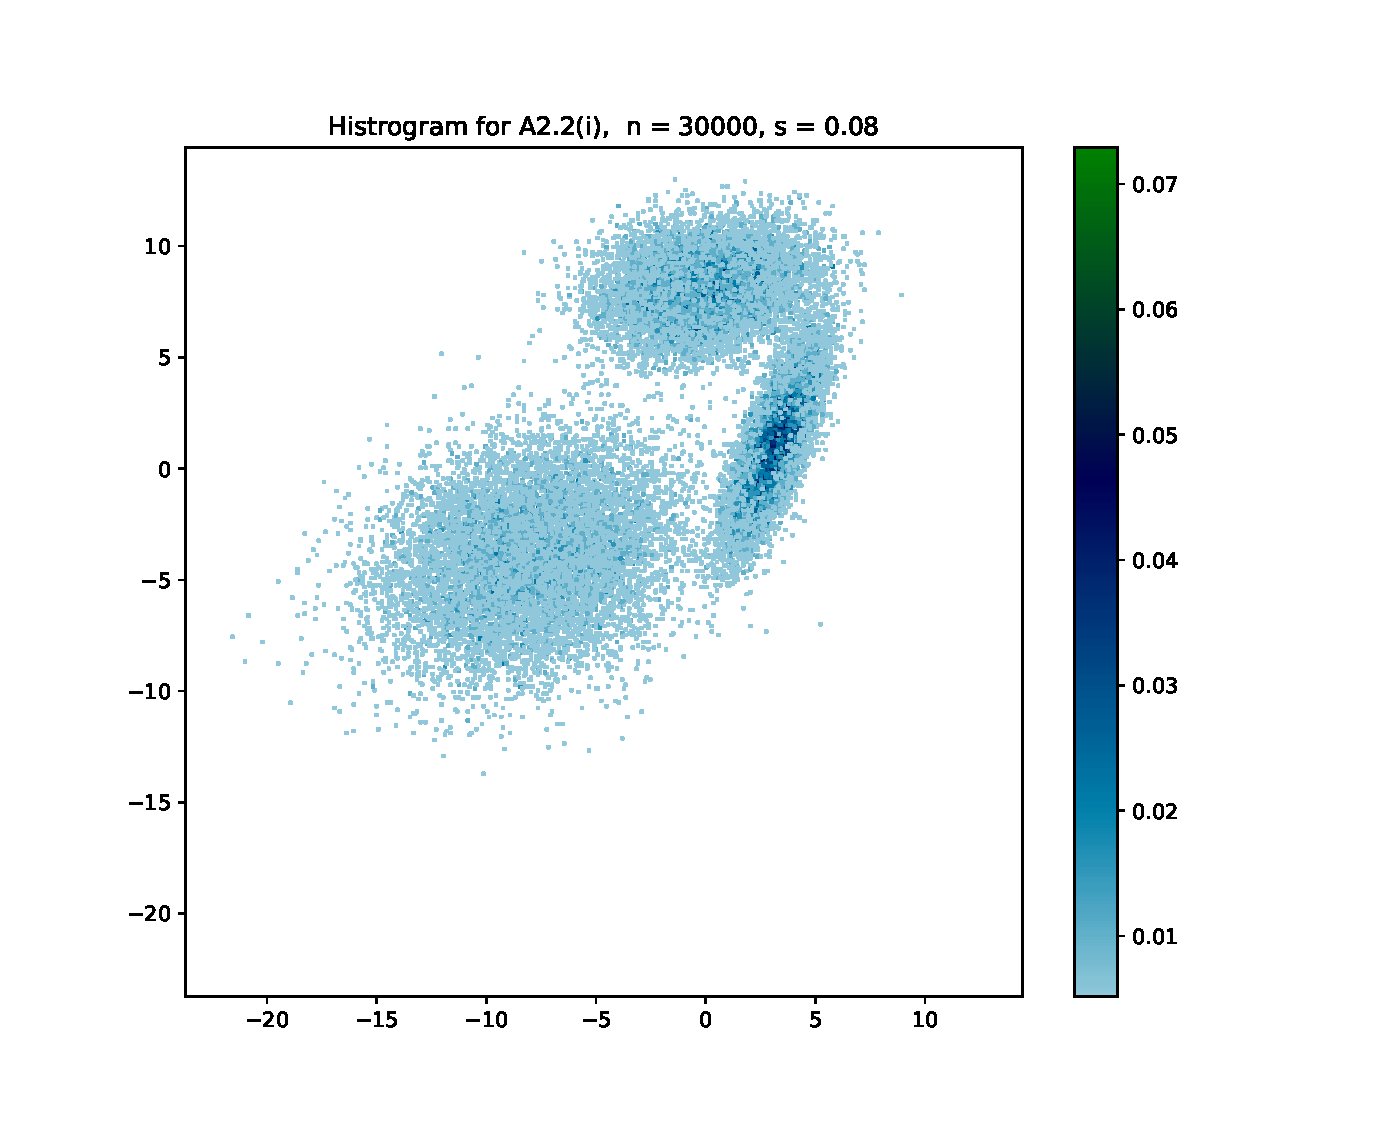
\includegraphics[height=8cm]{Figures_for_A2.2_i//10.eps}\\

\newpage
\textbf{Also we present our graphical results for Exercise 2.2 $ii)$:} \\
\hspace*{-1.5cm}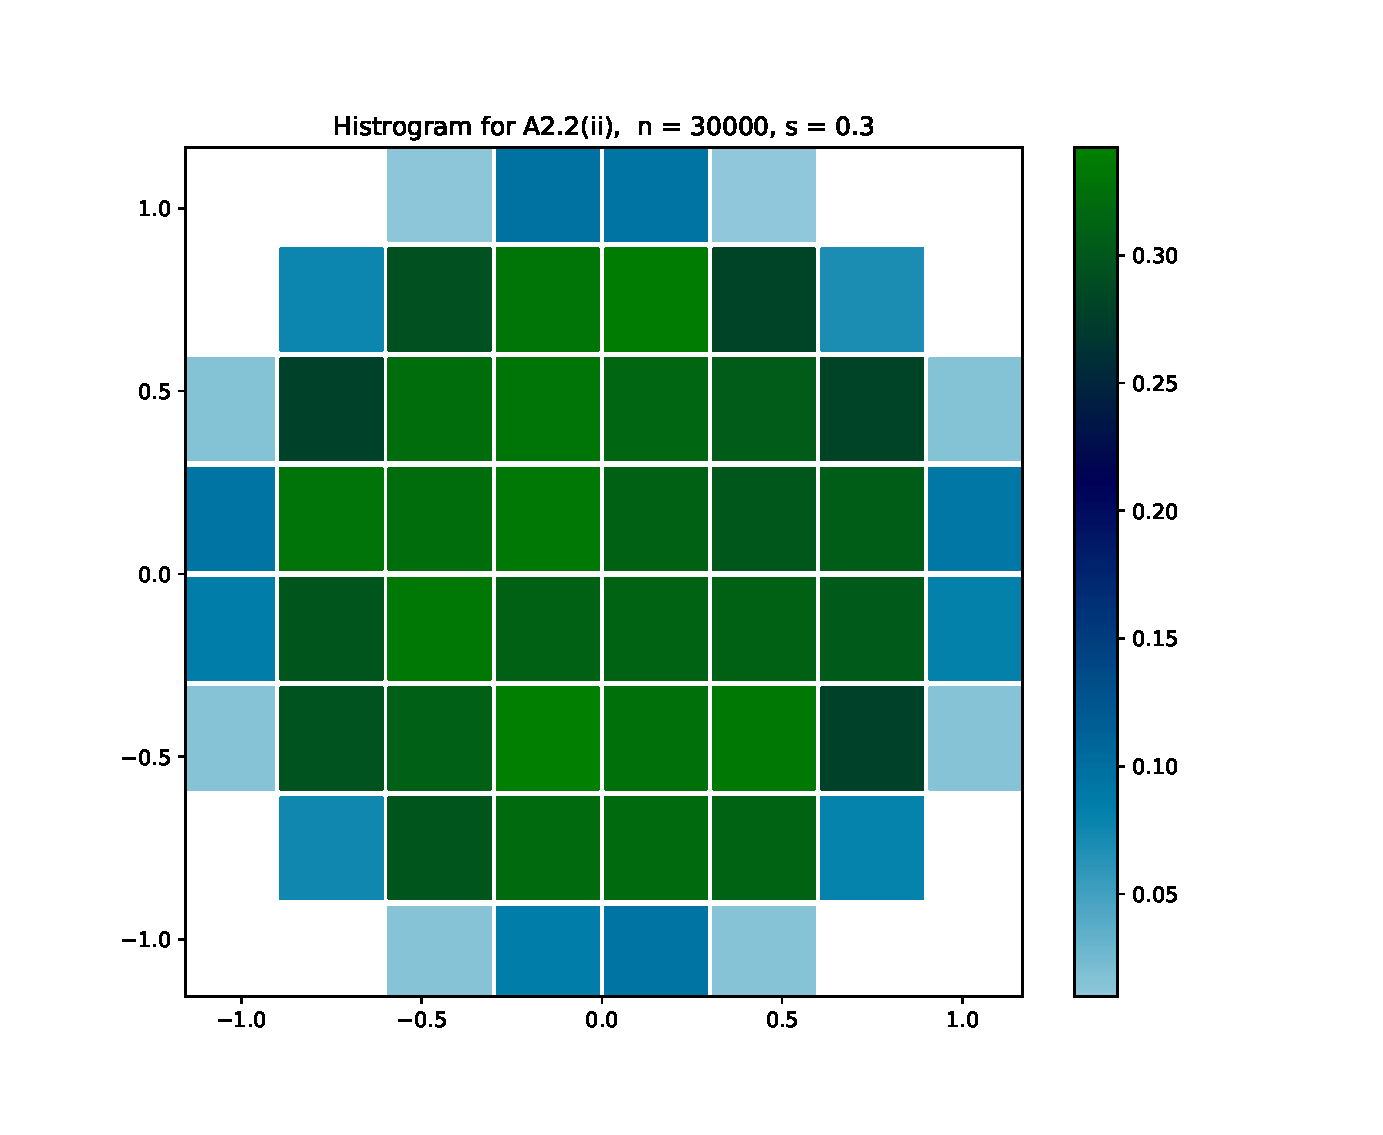
\includegraphics[height=8cm]{Figures_for_A2.2_ii//1.eps} \hspace*{-1.5cm}
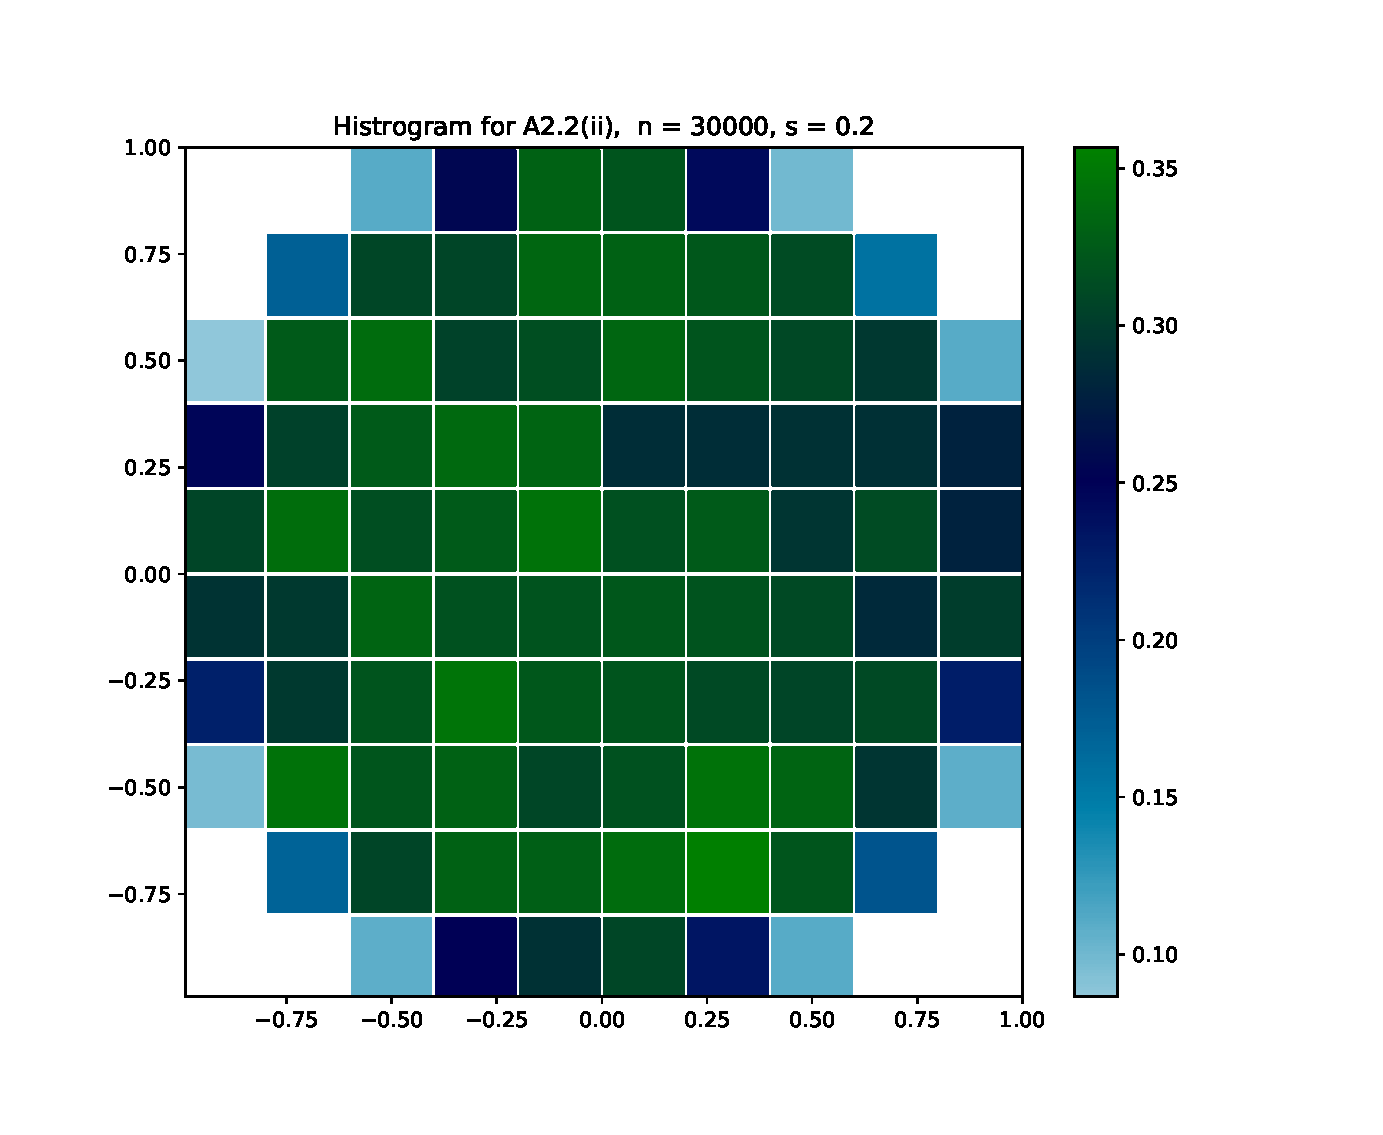
\includegraphics[height=8cm]{Figures_for_A2.2_ii//2.eps}\\
\hspace*{-1.5cm}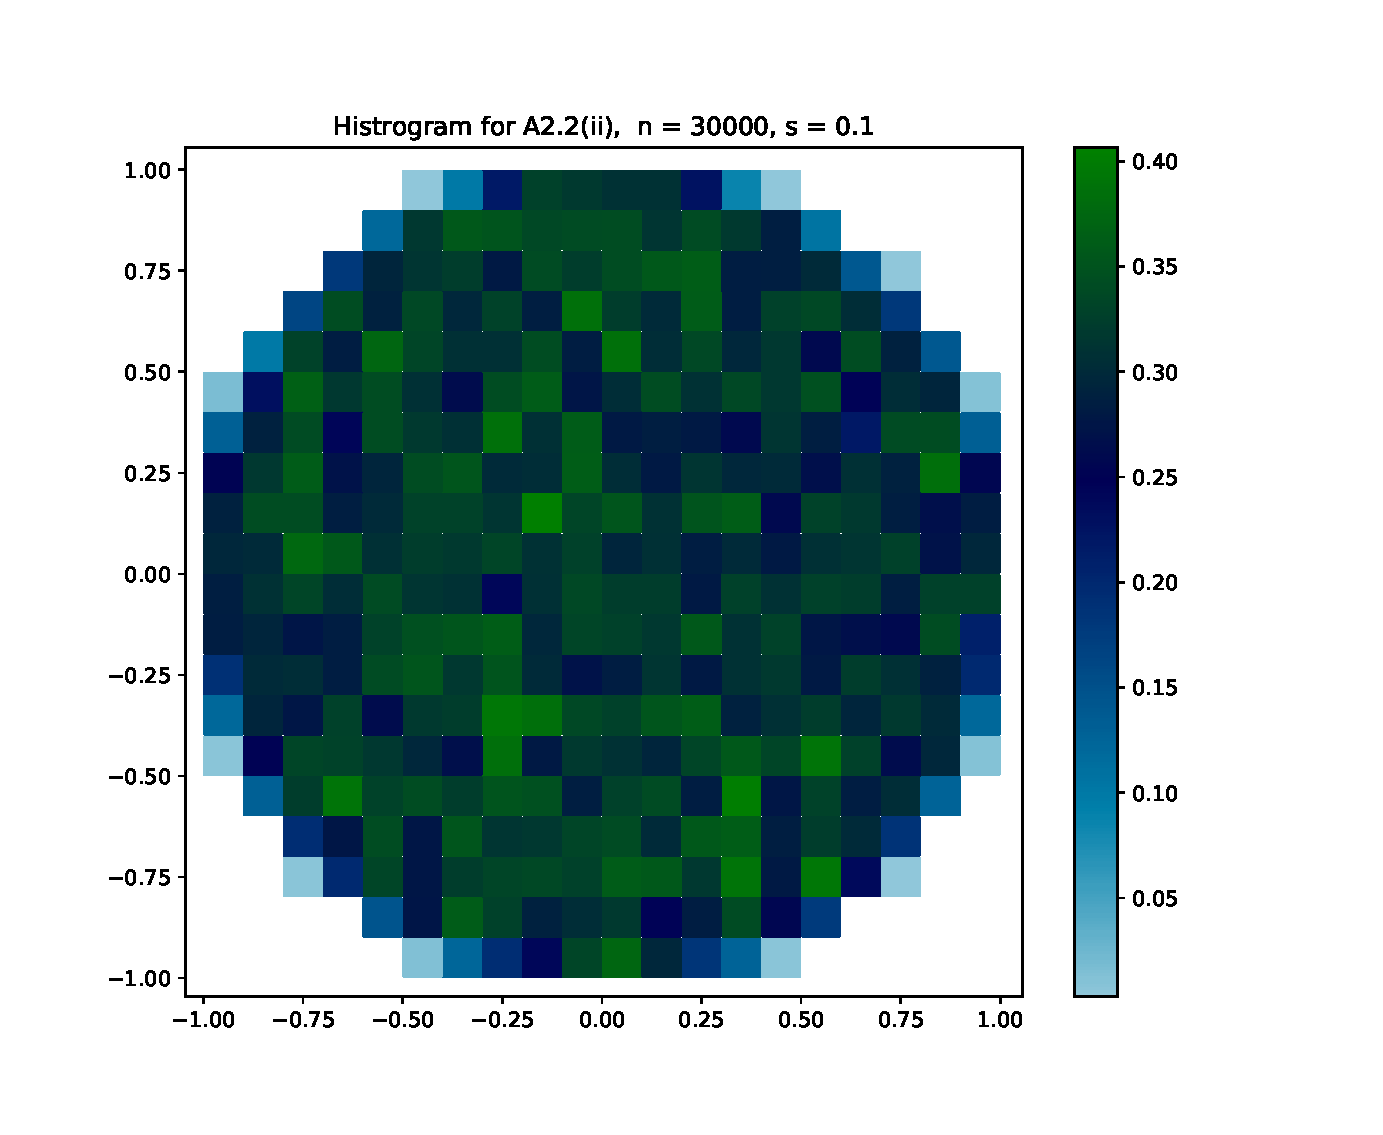
\includegraphics[height=8cm]{Figures_for_A2.2_ii//3.eps} \hspace*{-1.5cm}
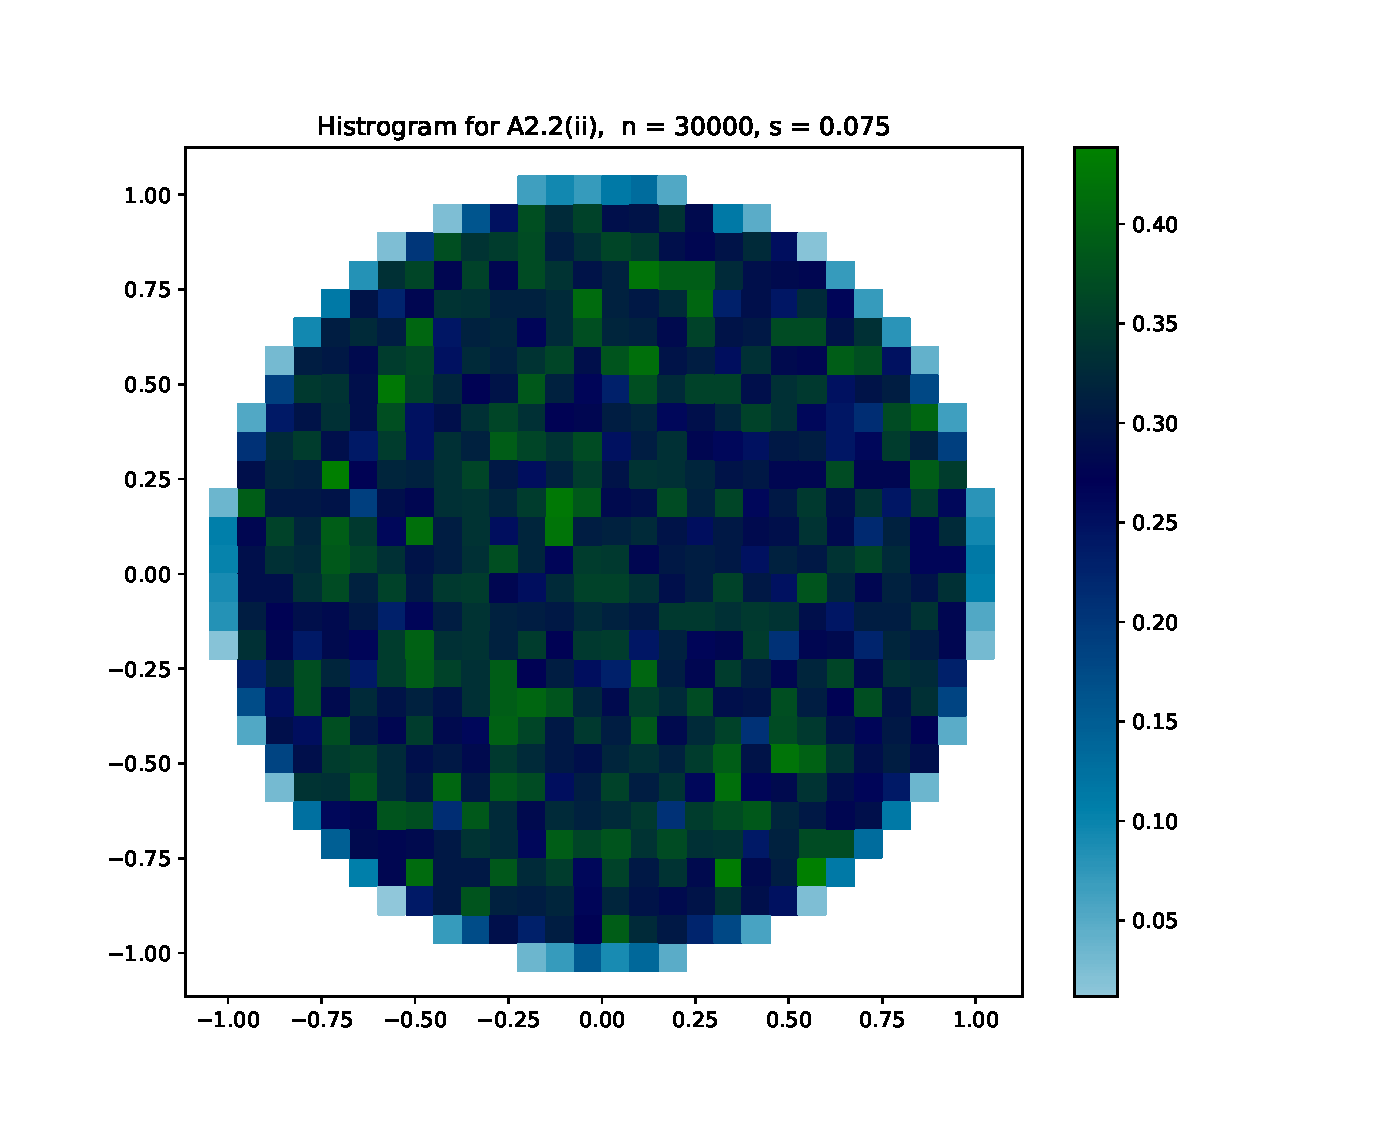
\includegraphics[height=8cm]{Figures_for_A2.2_ii//4.eps}\\
\hspace*{-1.5cm}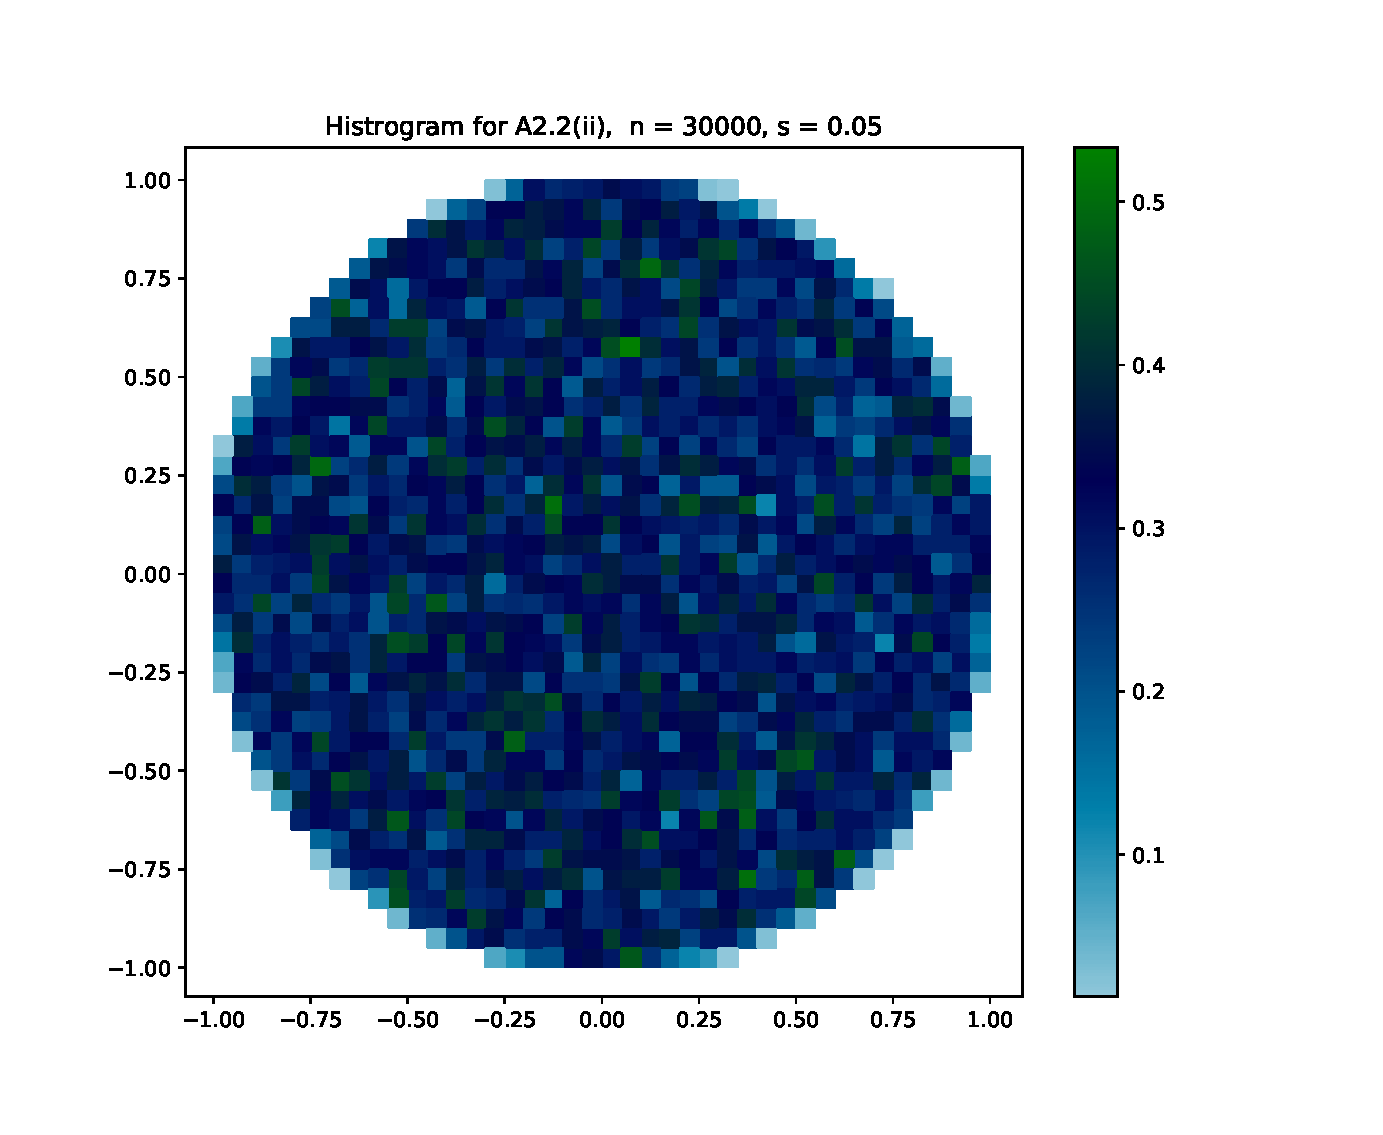
\includegraphics[height=8cm]{Figures_for_A2.2_ii//5.eps} \hspace*{-1.5cm}
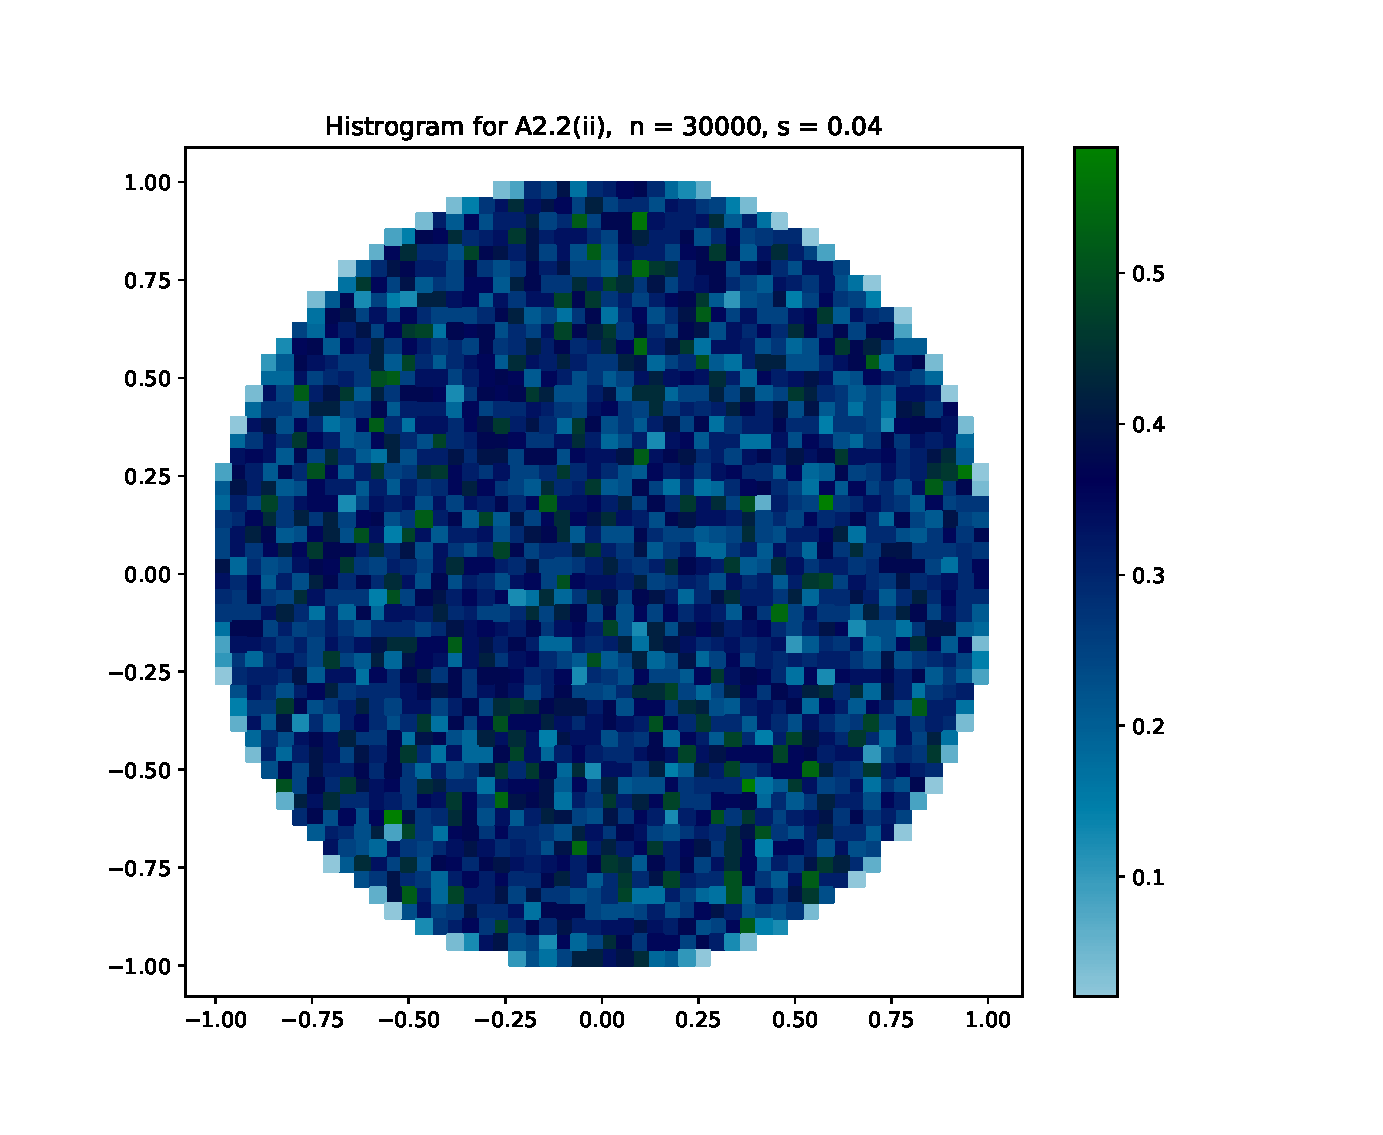
\includegraphics[height=8cm]{Figures_for_A2.2_ii//6.eps}\\
\hspace*{-1.5cm}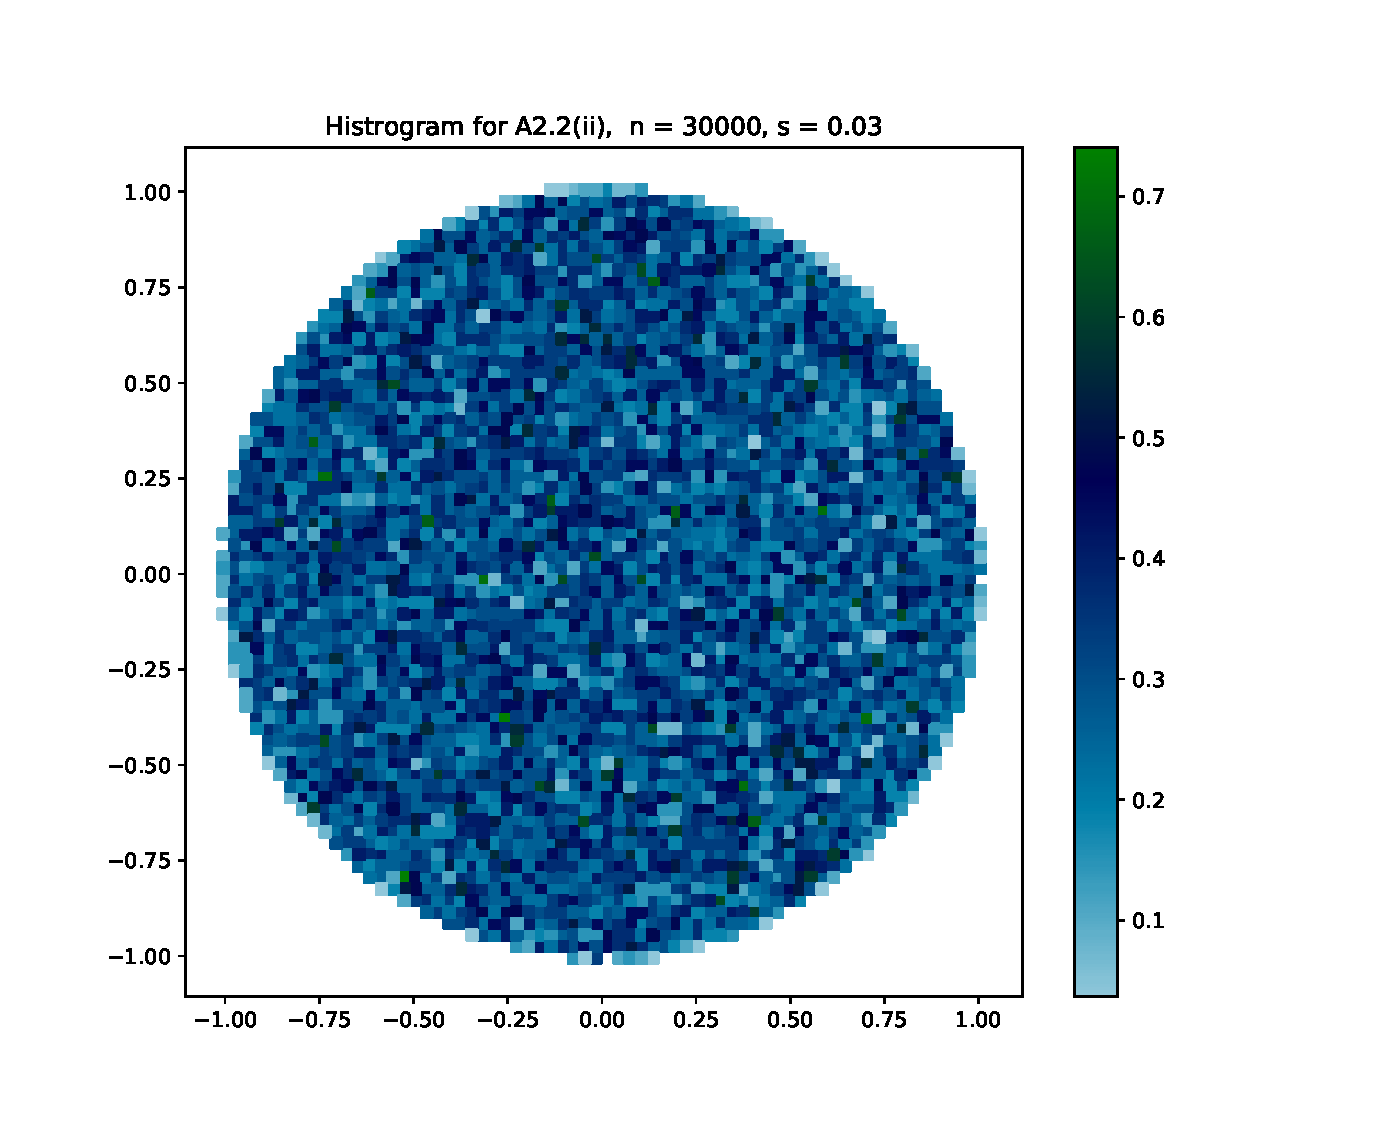
\includegraphics[height=8cm]{Figures_for_A2.2_ii//7.eps} \hspace*{-1.5cm}
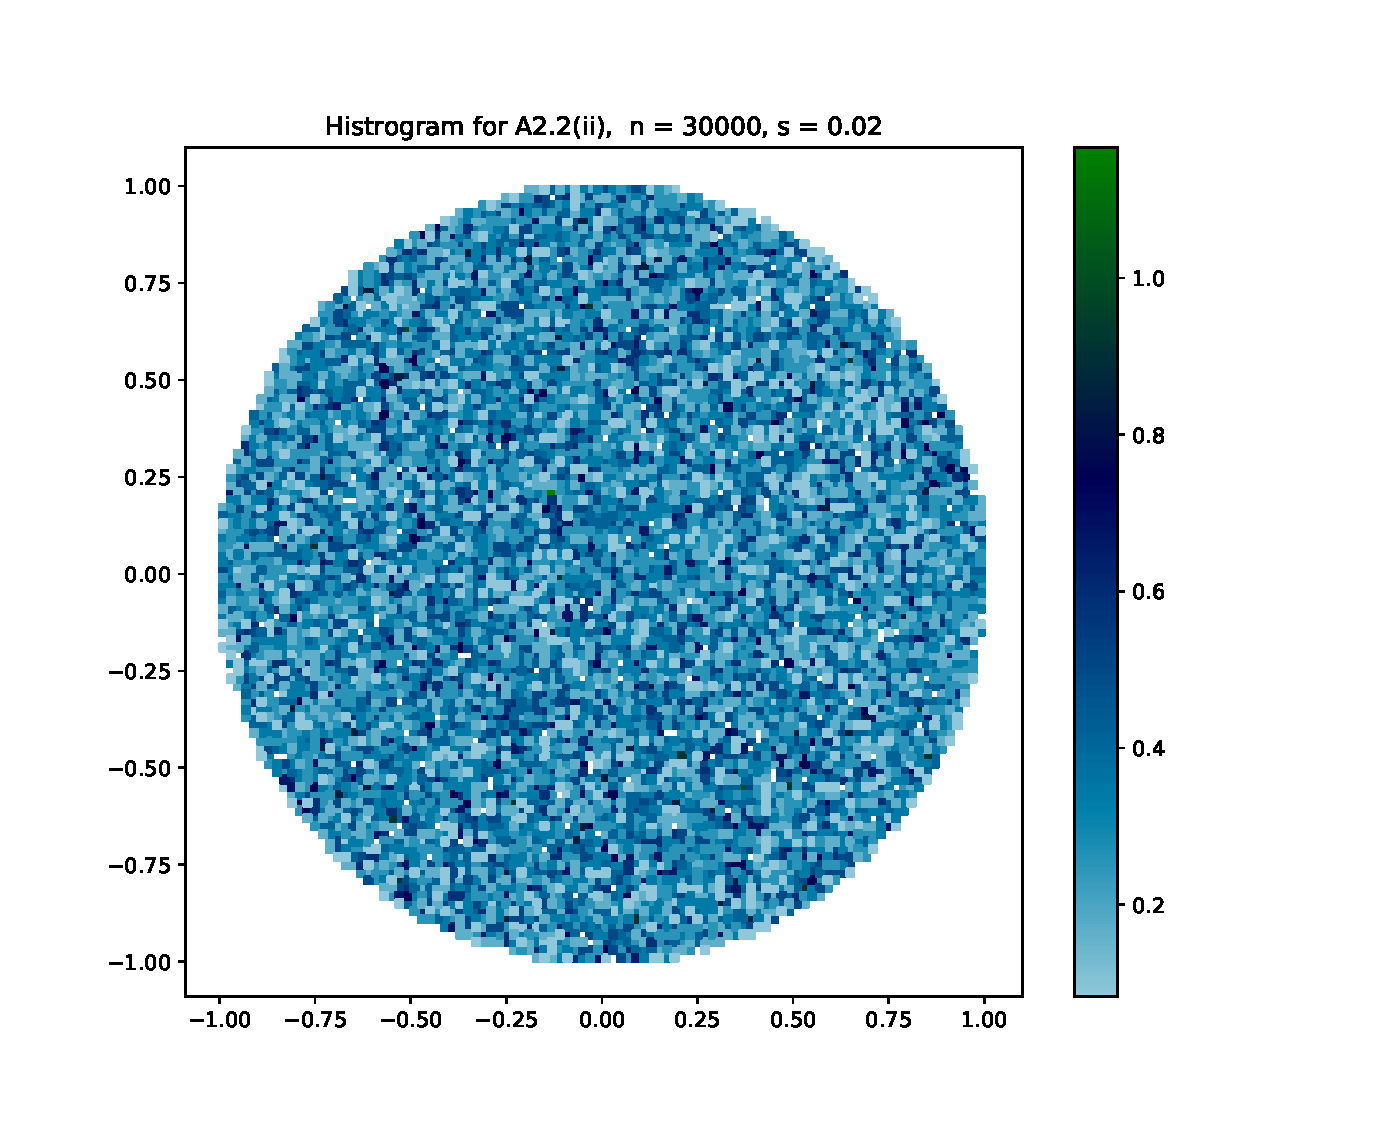
\includegraphics[height=8cm]{Figures_for_A2.2_ii//8.eps}\\
\hspace*{-1.5cm}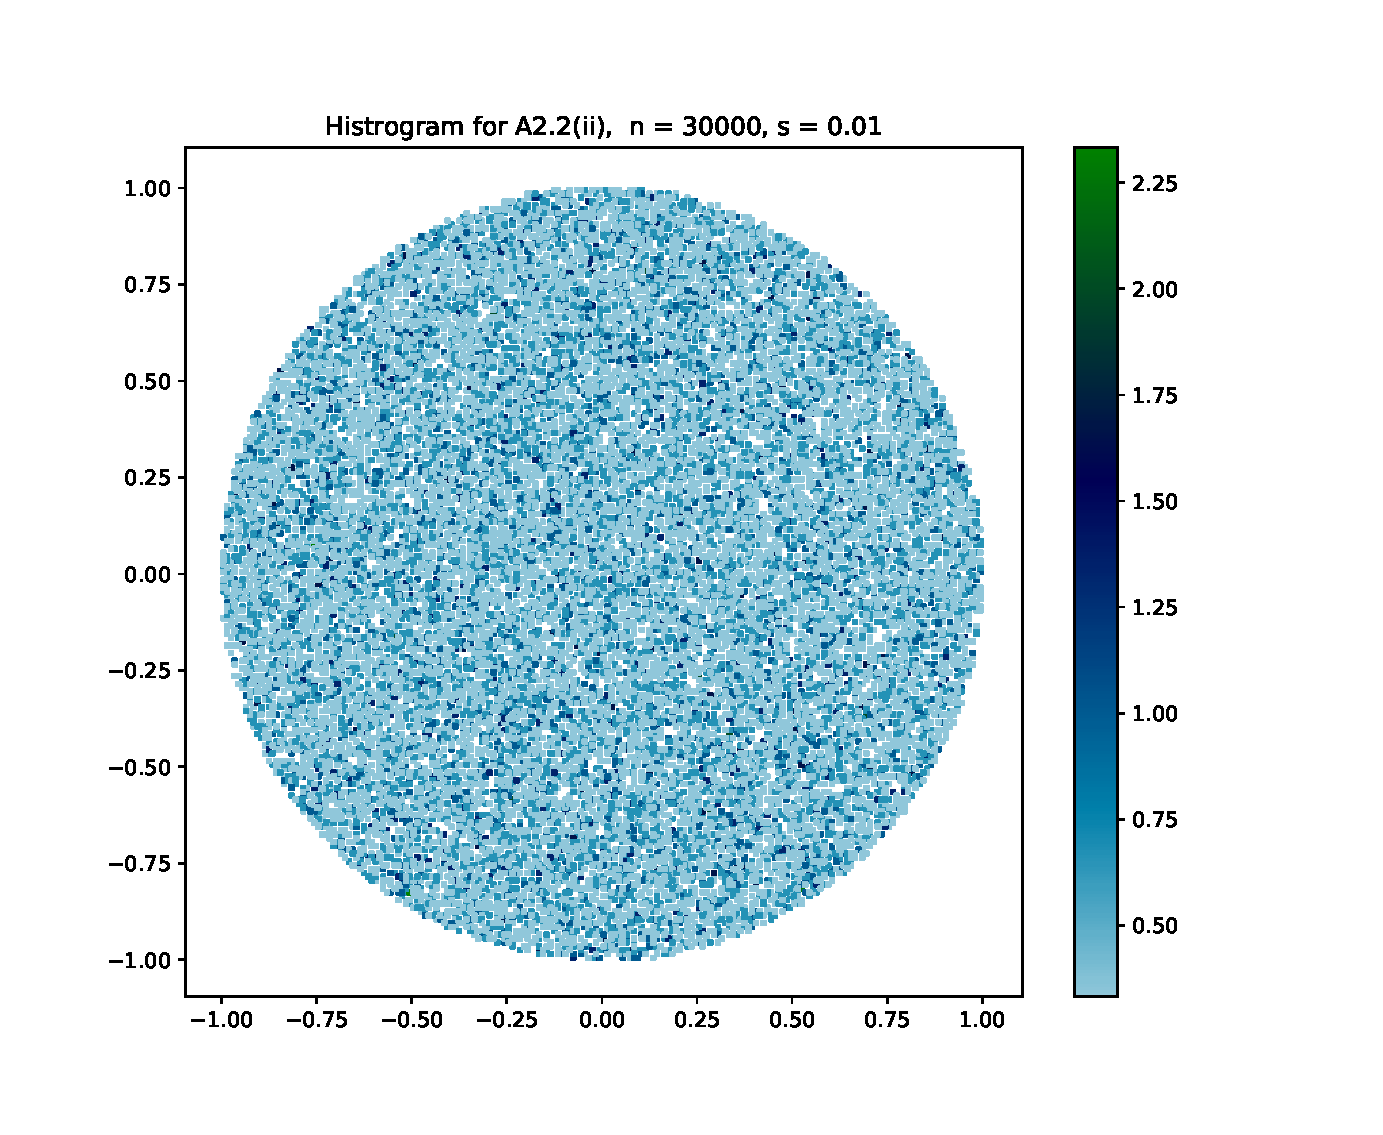
\includegraphics[height=8cm]{Figures_for_A2.2_ii//9.eps} \hspace*{-1.5cm}
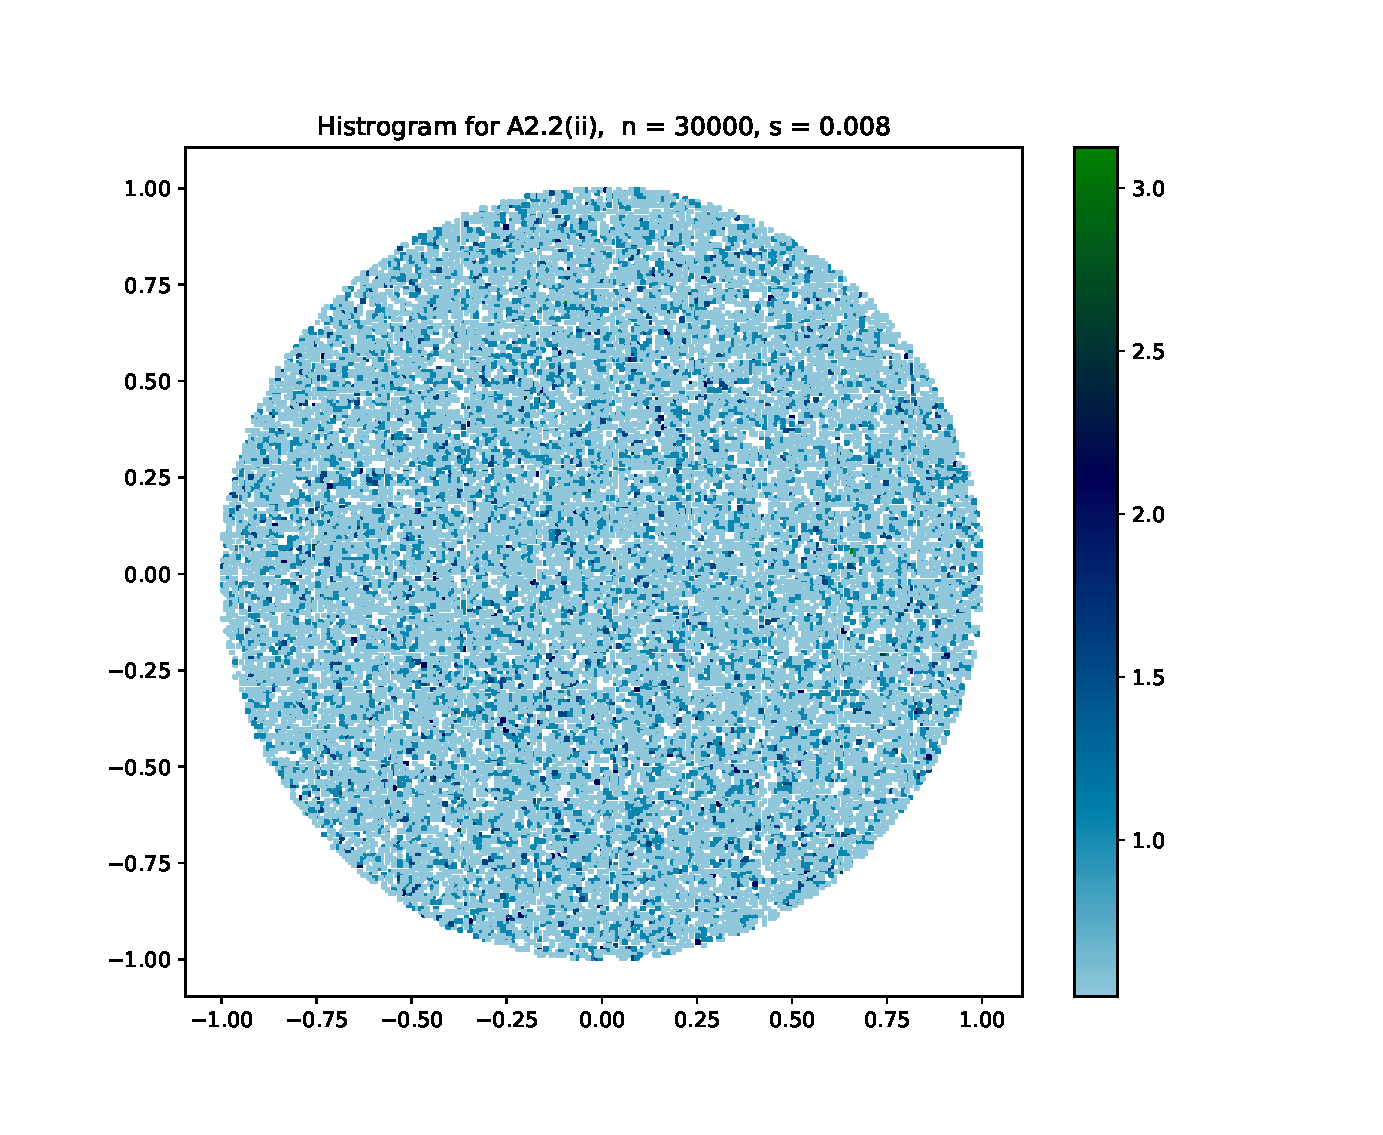
\includegraphics[height=8cm]{Figures_for_A2.2_ii//10.eps}\\








\end{document}